\documentclass[10pt]{standalone}
\usepackage[sc]{mathpazo}
\usepackage{commands}

\begin{document}
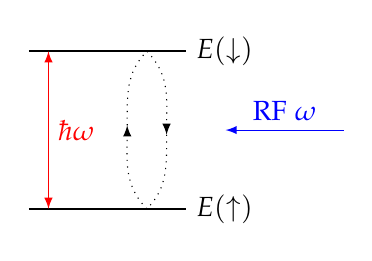
\begin{tikzpicture}
    \draw[thick] (0, 2) -- (2, 2);
    \draw[thick] (0, 0) -- (2, 0);
    \node[right] at (2, 2) {$E(\downarrow)$};
    \node[right] at (2, 0) {$E(\uparrow)$};
    \draw[red, latex-latex] (0.25, 0) -- (0.25, 2);
    \node[red, right] at (0.25, 1) {$\hbar\omega$};
    \draw[dotted, -latex] (1.5, 0) to [out=135,in=-90] (1.25, 1.06);
    \draw[dotted] (1.25, 1.06) to [out=90, in =-135] (1.5, 2);
    \draw[dotted, -latex] (1.5, 2) to [out=-45, in=90] (1.75, 0.94);
    \draw[dotted] (1.75, 0.94) to [out=-90, in=45] (1.5, 0);
    \draw[blue, -latex] (4, 1) -- (2.5, 1);
    \node[above, blue] at (3.25, 1) {RF $\omega$};
\end{tikzpicture}
\end{document}